\section{Parrot} \label{sec:parrot}

Although the latest advances on building stable
multi-threading systems are promising, whether \smt systems can be 
made simple and deployable stills remains an open challenges. Existing systems 
either incur high performance overhead~cite{dthreads:sosp11} (For instance, 
we observed
that a prior system, \dthreads, had 5$\times$ to 100$\times$ slowdown on
some programs), or require sophiscated
program analysis~cite{peregreine:sosp11, bergan:oopsla13} and fairly hard to 
deploy.
These limitations make evaluation in existing systems limited: they often 
used (1) synthetic benchmarks,
not real-world programs, from incomplete benchmark suites; (2) one workload
per program; and (3) at most 8 cores (with three exceptions; see \S\ref{sec:
related}).

These limitations are intermingled.  Reducing schedules improves correctness
but trades performance because the schedules left may not balance each
thread's load well, causing some threads to idle unnecessarily.  Our
experiments show that ignoring load imbalance as in \dthreads
can lead to pathological
slowdown if the order of operations enforced by a schedule
\emph{serializes} the intended parallel computations
(\S\ref{sec:comparison}).  To recover performance, one method is to count
the instructions executed by each thread and select schedules that balance
the instruction counts~\cite{kendo:asplos09, coredet:asplos10,
  dmp:asplos09}, but this method is not stable because input or program
perturbations easily change the instruction counts.  The other method (we 
proposed)
lets the nondeterministic OS scheduler select
a reasonably fast schedule and reuses the schedule on
compatible inputs~\cite{cui:tern:osdi10,peregrine:sosp11}, but it
requires sophisticated program analysis, complicating deployment.

We present \parrot,\footnote{We name our system after one of the most
  trainable birds.} a simple, deployable runtime that efficiently makes
threads deterministic and stable by offering a new contract to developers.
By default, it schedules synchronizations in each thread using
round-robin, vastly reducing schedules and providing broad repeatability.
When default schedules are slow, it allows advanced developers to add
intuitive \emph{performance hints} to their code for speed.  Developers 
discover
where to add hints through profiling as usual, and \parrot simplifies
performance debugging by deterministically reproducing the bottlenecks.
The hints are robust to developer mistakes as they can be safely ignored
without affecting correctness.

Like prior systems, \parrot's contract reduces schedules to favor correctness 
over performance.  Unlike prior systems, it allows advanced developers
to optimize performance.  We believe this practical ``meet in the
middle'' contract eases writing correct, efficient programs.

% based on several years of lessons.

%% Like prior systems, \parrot's contract favors correctness over performance
%% by vastly reducing schedules.  Unlike prior systems, it provides
%% advanced developers the flexibility for better performance.

\parrot provides two performance hint abstractions.  A \emph{soft
  barrier} encourages the scheduler to coschedule a group of threads at
given program points.  It is for performance only, and operates as a
barrier with deterministic timeouts in \parrot.  Developers use it to switch
to faster schedules without compromising determinism
when the default schedules serialize parallel
computations (\S\ref{sec:example}).  A \emph{performance critical section}
informs the scheduler that a code region is a potential
bottleneck, encouraging the scheduler to get through the region fast.
When a thread enters a performance critical section, \parrot delegates 
scheduling to the
nondeterministic OS scheduler for speed.  
Performance critical sections may trade some determinism for
performance, so they should be applied only when the schedules they add
are thoroughly checked by tools or advanced developers.
These simple abstractions
let \parrot run fast on all programs evaluated, and
may benefit other DMT or \smt systems and classic nondeterministic
schedulers~\cite{coschedule:sigmetrics96, coschedule, partial-barrier:atc06}.

Our \parrot implementation is \pthread-compatible, simplifying deployment.
It handles many diverse constructs real-world programs depend upon such as
network operations and timeouts.  \parrot makes synchronizations outside
performance critical sections deterministic but allows nondeterministic
data races.  Although it is
straightforward to make data races deterministic in \parrot,
% with a memory commit protocol we designed, 
we deemed it not worthwhile because the cost of doing so outweighs the
benefits (\S\ref{sec:discussion}).  \parrot's determinism is similar to
\kendo's weak determinism~\cite{kendo:asplos09}, but \parrot offers stability
which Kendo lacks.

Third, we quantitatively show that \parrot achieves good performance and high
model checking coverage on a diverse set of \nprog programs.  The programs
include \nrealprog real-world programs, such as \bdb~\cite{berkeleydb},
\openldap~\cite{openldap}, \redis~\cite{redis}, \mplayer~\cite{mplayer},
all \nstl parallel C++ STL algorithm 
implementations~\cite{parallel-stl} which use \openmp, and all \nimagick
parallel image processing utilities (also \openmp) in the \imagick~\cite{
imagick}
software suite.  Further, they
include \emph{all} \nbenchmarks programs in four widely used benchmark suites:
\parsec~\cite{parsec}, \phoenix~\cite{phoenix-benchmarks}, \splashx~\cite{
splashx},
and \npb~\cite{npb}.  We used complete software or benchmark suites to
avoid biasing our results. The programs together cover many different
parallel programming models and idioms such as threads,
\openmp~\cite{openmp}, fork-join, map-reduce, pipeline, and workpile.  To
our knowledge, our
evaluation uses roughly \overeach more programs than any prior
DMT or \smt evaluation, and \overcombined more than all
prior evaluations combined.
% We used at least three different scales/types of workloads per program
% and a 24-core machine to make our results robust.
Our experiments show:

\begin{enumerate}

\item[$\bullet$] \parrot is easy to use. It averages only \hintsperprog lines of hints
  per program to get good performance, and adding hints is fast.  Of all
  \nprog programs, \nprognohints need no hints, \nproglineuphints need
  \computes which do not affect determinism, and only \nprognondethints
  programs need \nondets to trade some determinism for speed.

\item[$\bullet$] \parrot has low overhead.  At the maximum allowed (16--24) cores, \parrot's
  geometric mean overhead is \meanrealoverhead for \nrealprog real-world 
programs,
  \meanbenchoverhead for the other \nbenchmarks programs, and \meanoverhead 
for all.

\item[$\bullet$] On \nprogcompared programs that two prior systems \dthreads~\cite{
dthreads:sosp11}
  and \coredet~\cite{coredet:asplos10} can both handle, \parrot's overhead is \
xxxcompoverhead whereas \dthreads's
  is \dthreadssyncoverhead and \coredet's \coredetoverhead.

\item[$\bullet$] \parrot scales well to the maximum allowed cores on our 24-core server and
  to at least three different scales/types of workloads per program.

\end{enumerate}

\subsection{Evaluation} \label{sec:parrot-eval}

We evaluated \parrot on a diverse set of \nprog programs. This set
includes \nrealprog real-world programs: \bdb, a widely used database
library~\cite{berkeleydb}; \openldap, a server implementing the
Lightweight Directory Access Protocol~\cite{openldap}; \redis, a fast
key-value data store server~\cite{redis}; \mplayer, a popular media
encoder, decoder, and player~\cite{mplayer}; \pbzip, a parallel
compression utility~\cite{pbzip2}; \pfscan, a parallel \v{grep}-like
utility~\cite{pfscan}; \aget, a parallel file download
utility~\cite{aget}; all \nstl parallel C++ STL algorithm
implementations~\cite{parallel-stl} which use \openmp; all \nimagick
parallel image processing utilities (which also use \openmp) in the
\imagick software suite~\cite{imagick} to create, edit, compose, or
convert bitmap images.  The set also includes all \nbenchmarks programs in
four widely used benchmark suites including \nparsec in
\parsec~\cite{parsec}, \nphoenix in
\phoenix~\cite{phoenix-benchmarks}, \nsplash in
\splashx~\cite{splashx}, and \nnpb in \npb~\cite{npb}.  The \phoenix
benchmark suite provides two implementations per algorithm, one using
regular Pthreads (marked with \v{-pthread} suffix) and the other using
a map-reduce library atop Pthreads.  We used complete software or
benchmark suites to avoid biasing our results.  The programs together
cover a good range of parallel programming models and idioms such as
threads, \openmp, data partition, fork-join, pipeline, map-reduce, and
workpile.  To the best of our knowledge, our evaluation of \parrot
represents \overeach more programs than any prior DMT or \smt
evaluation, and \overcombined more than all prior
evaluations combined.

Our evaluation machine was a 2.80 GHz dual-socket hex-core Intel Xeon
with 24 hyper-threading cores and 64 GB memory
running Linux 3.2.14.  Unless otherwise specified, we used the maximum
number of truly concurrent threads allowed by the machine and programs.  For 83
out of the \nprog programs, we used 24.  For 13 programs, we used 16
because they require the number of threads be a power of 
two. For \ferret, we used 18 because it requires
the number of threads to be 4$n$+2. For \mplayer, we used 8,
the max it takes. For the other
10 programs, we used 16 because they reach peak performance with
this thread count.  In scalability experiments, we varied the number of
threads from 4 to the max.



Unless otherwise specified, we used the following workloads.  For \bdb, we
used a popular benchmark \v{bench3n}~\cite{benchthreen}, which does
fine-grained, highly concurrent transactions. For both \openldap and
\redis, we used the benchmarks the developers themselves use, which come
with the code. For \mplayer, we used its utility \mencoder to transcode a
255 MB video (OSDI '12 keynote) from MP4 to AVI.  For \pbzip, we
compressed and decompressed a 145 MB binary file.  For \pfscan, we searched for
the keyword \v{return} in all 16K files in \v{/usr/include} on our
evaluation machine.  For \aget, we downloaded a 656 MB file. For all
\imagick programs, we used a 33 MB JPG.  For all \nstl
parallel STL algorithms, we used integer vectors with 4G elements.  For
\parsec, \splashx, and \phoenix, we used the largest workloads
because they are considered ``real'' by the benchmark authors.  For \npb, we
used the second largest workloads because the largest workloads are intended 
for
supercomputers. In workload sensitivity experiments, we used workloads of
3 or 4 different scales per program, typically with a 10$\times$ difference 
between
scales.  We also tried 15 different
types of workloads for \redis and 5 for \mplayer.  All workloads ran from
a few seconds to about 0.5 hour, using 100 or 10
repetitions respectively to bring the standard error below 1\%.
All overhead means are geometric.

We compiled all programs using \v{gcc -O2}.  To support
\openmp programs such as parallel STL algorithms, we used the GNU \libgomp.
When evaluating \parrot on the client program \aget and the server programs \
openldap
and \redis, we ran both endpoints on the same machine to avoid network
latency.  \nprogadhocsync programs use ad hoc
synchronization~\cite{syncfinder:osdi10}, and we added a \v{sched\_yield}
to the busy-wait loops to make the programs work with \parrot.  \nprogtimeout
programs use \pthread timed operations, and we added \v{set\_base\_time}
(\S\ref{sec:timeout}) to them. We set the spin-wait of \parrot's scheduler
to $10^5$ cycles.  We used the default \compute timeout of 20 except 3,000
for \ferret.  Some \phoenix programs read large files, so
we ran them with a warm file cache to focus on measuring their computation
time. (Cold-cache results are unusable due to large
variations~\cite{Parrot:github}.)


The rest of this section focuses on these questions:
\begin{enumerate}

\item[\S\ref{sec:ease-of-use}:] Is \parrot easy to use?  How many hints are
  needed to make the programs with \parrot fast?

\end{enumerate}





\subsection{Ease of Use} \label{sec:parrot-use}

Of all \nprog programs, \nprognohints have reasonable overhead with
default schedules, requiring no hints.  \nproglineuphints programs need a 
total of 
\nlineofcomputehints lines of \compute hints: \nproggenericlineuphints
need only 4 lines of generic \compute hints in \libgomp, and
\nprogspecificlineuphints need program-specific \computes
(Table~\ref{tab:computehints}).  These programs enjoy both determinism and
reasonable performance.  Only \nprognondethints programs 
need a total of \nlineofnondethints lines of \nondet hints to
trade some determinism for performance (Table~\ref{tab:nondethints}).
On average, each program needs only \hintsperprog lines.


In our experience, adding hints was straightforward.  It took roughly 0.5--2 
hours per program despite unfamiliarity with the programs.  We believe
the programs' developers would spend much less time adding better hints.
\parrot helped us deterministically reproduce the bottlenecks and identify
the synchronizations delayed by round-robin.  We used Intel \vtune~\cite{vtune} and
Linux \v{perf}~\cite{perf} performance counter-based tools to identify time-
consuming computations, and usually needed to align only the top two or three
computations.  For instance, \ferret uses a pipeline of six stages, all
serialized by the \parrot's default schedules.  We aligned only two of them to 
bring the overhead down to a reasonable level.  Aligning more stages did not help.










\begin{table}[t]
\footnotesize
\centering
\begin{tabular}{lr}
{\bf Program} & {\bf Lines} \\
\hline

\mencoder, \vips, \swaptions, \freqmine, \facesim
,                                 &   2 each  \\
\xtwosixfour, \radiosity, \radix, \kmeans, \\
\linearregrepthread, \linearregre, \\
\matrixmultpthread, \matrixmult, \\
\wordcntpthread, \stringmatchpthread, \\
\stringmatch, \histogrampthread, \histogram \\

\hline

\pbzip, \ferret,                                  &   3 each   \\
\kmeanspthread, \pcapthread, \pca, \wordcnt \\

\hline

\libgomp, \bodytrack  &   4 each  \\

\hline

\imagick (12 programs)                          &   25 total  \\

\end{tabular}
\caption{{\em Stats of \compute hints.} \nproglineuphints
  programs need \compute hints.  The hints in \libgomp benefit all \openmp
  programs including \imagick, STL, and \npb.} \label{tab:computehints}
\end{table}

\begin{table}[t]
\footnotesize
\centering
\begin{tabular}{lrl}
{\bf Program} & {\bf Lines} & {\bf Nondet Sync Var} \\
\hline

\pfscan                       &   2   &   \v{matches\_lock}   \\

\partition                &   2  &   \v{\_\_result\_lock}   \\

%% mutex array name: mutex[][].
\fluidanimate          &   6  &   \v{mutex[i][j]} \\

%% mutex array name: lock_array[].
\fmm                  &   2   &  \v{lock\_array[i]} \\

%% mutex array name: tasks[i].taskLock, i is thread id.
\cholesky             &   2   &  \v{tasks[i].taskLock} \\
\raytrace             &   2   &  \v{ridlock}   \\

%% mutex array name: tlock[].
\ua                       &   6   &  \v{tlock[i]} \\

\end{tabular}
\caption{{\em Stats of \nondet hints.} \nprognondethints programs need \nondet
  hints. The hints in \partition are generic for three STL programs
  \partition, \nthelement, and \partialsort. The last column shows the
  synchronization variables whose operations are made
  nondeterministic.} \label{tab:nondethints}
\end{table}

\subsection{Performance} \label{sec:parrot-performance}

\begin{figure*}[tb]
\centering
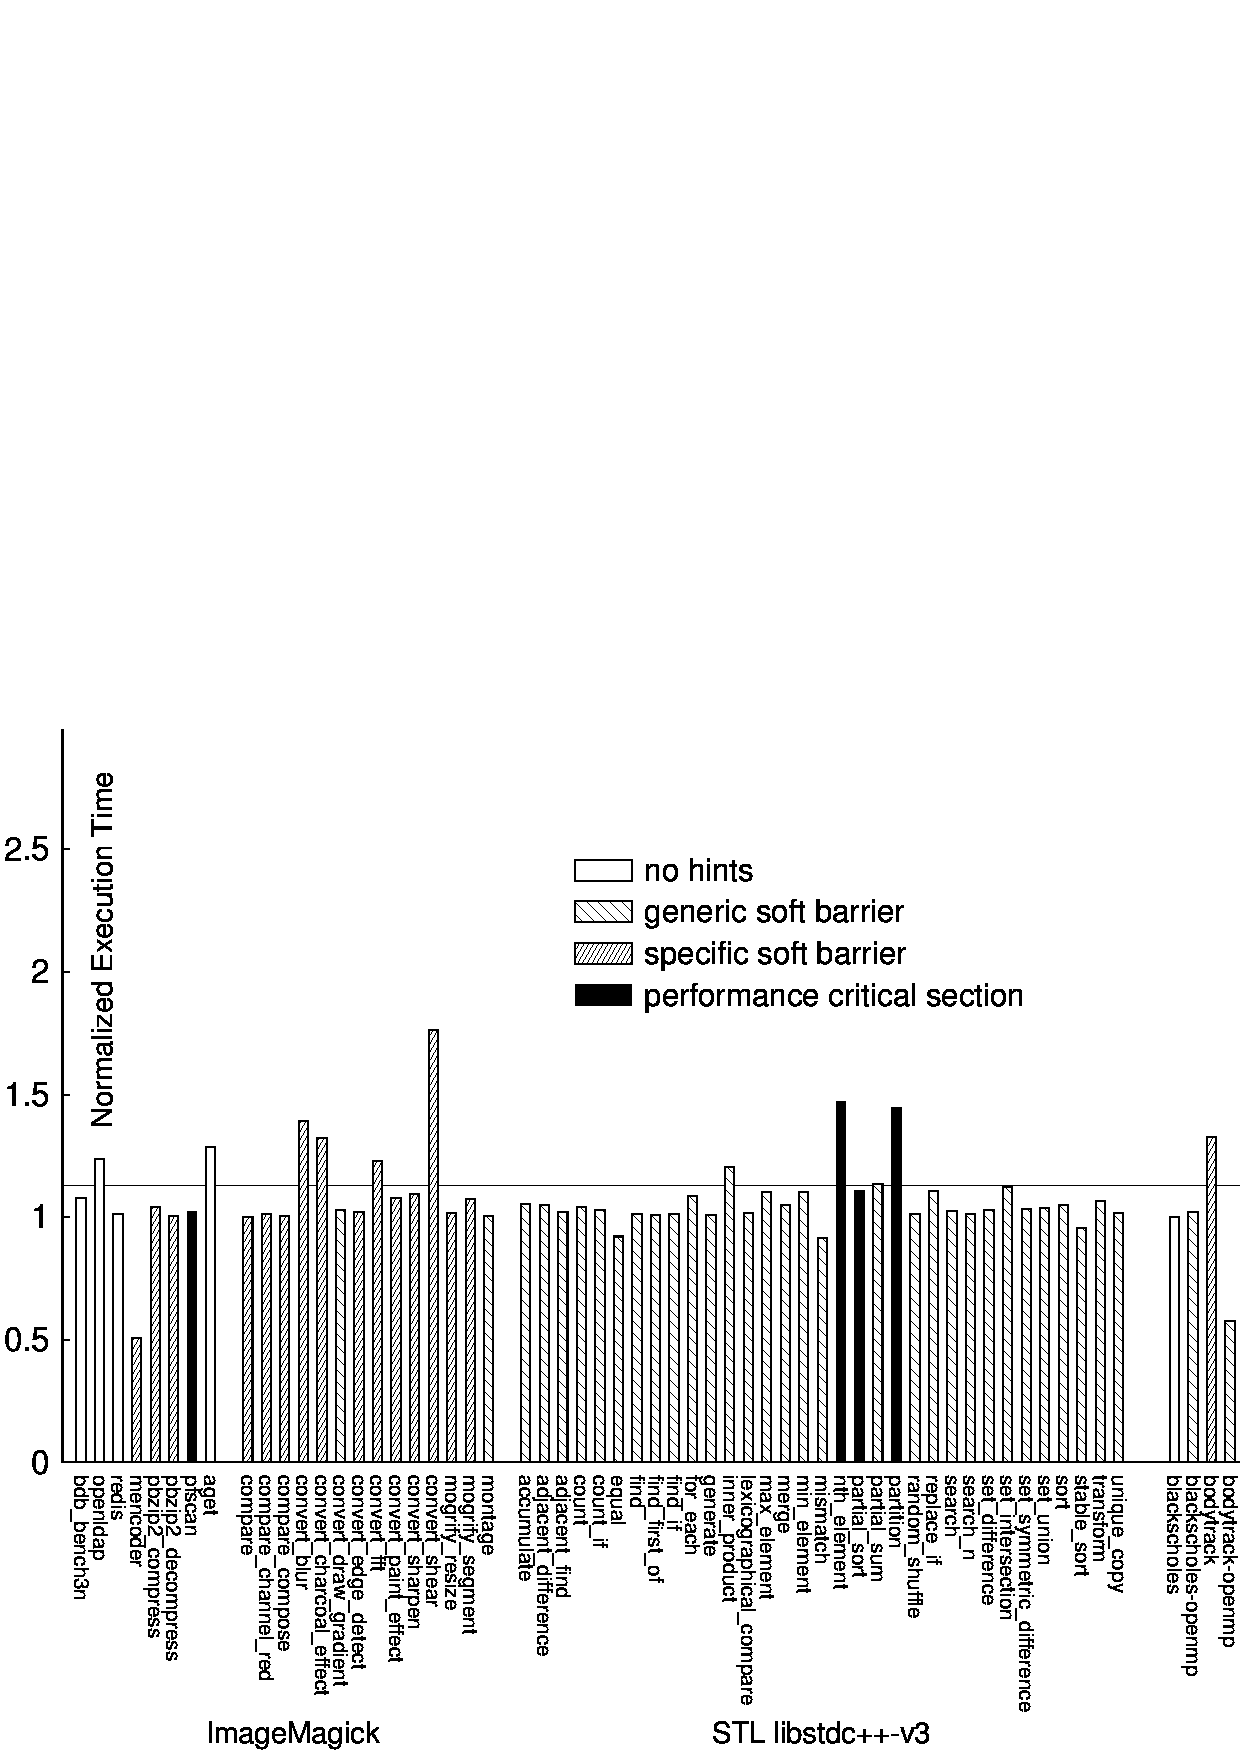
\includegraphics[width=\textwidth]{parrot/figures/overhead}
\vspace{-.20in}
\caption{{\em \parrot's performance normalized over nondeterministic
    execution.}  The patterns of the bars show the types of the hints the 
programs
  need: no hints, generic \computes in \libgomp, program-specific
  \computes, or \nondets.  The mean overhead is
  \meanoverhead (indicated by the horizontal line).} \label{fig:overhead}
\vspace{-.05in}
\end{figure*}

Figure~\ref{fig:overhead} compares \parrot's performance to nondeterministic
execution.  Even with the maximum number of threads (16--24), the mean
overhead is small: \meanrealoverhead for real-world programs, \
meanbenchoverhead for benchmark
programs, and \meanoverhead for all programs.
Only seven programs had over 100\% overhead.  The \ferret, \freqmine, and \is 
benchmarks
had dynamic load imbalance even with the starting points of the computations
aligned with \compute hints. \ua also had load 
imbalance even after \nondet hints are added.
\xtwosixfour is a pipeline program, and its overhead
comes from the \compute timeouts during the pipeline startup and
teardown.  \rtviewraytrace and \barnes have low-level
synchronizations in tight loops, and their overhead may be further reduced
with \nondets.  Four programs, \mencoder, \bodytrackopenmp, \facesim, and
\linearregrepthread, enjoyed big speedups, so we analyzed their 
executions with profiling tools. We found that the number of \mencoder's 
context switches due to synchronization decreased from 1.9M with
nondeterministic executions to 921 with \parrot.  The reason of the context
switch savings was that \parrot's round-robin scheduling reduced contention
and its synchronizations use a more efficient wait that combines spin- and
block-waits (\S\ref{sec:scheduler}).  \bodytrackopenmp and \facesim
enjoyed a similar benefit.  So did another 19 programs which had
10$\times$ fewer context switches with
\parrot~\cite{Parrot:github}. \linearregrepthread's stalled cycles were
reduced by 10$\times$ with \parrot, and we speculate that \parrot's scheduler
improved its affinity. (See~\cite{Parrot:github} for all results on
microarchitectural events.)



